 \chapter{The Frangi Filter: A multiscale approach} \label{sec:frangi-multiscale}
    
     With the ideas of scale established, we may return to our discussion of the Frangi filter.
    Our ideas of scale developed in the previous section imply that, if the ridgelike structures we wish to detect are more prominent at different scales, then a multiscale approach is the natural one. Considering our
    developments in \cref{sec:frangi}, we wish to probe at multiple scales
    regions that would receive a high vesselness score at any range,
    and consider them all together. Frangi \cite{frangi-paper} approached this problem by simply taking the maximum vesselness measure over all scales. Thus the multiscale Frangi vesselness score at the pixel $(x_0, y_0$) would be 
    
    \begin{equation} \label{eq:Vmax}
    \Vmax(x_0, y_0) =
    	\underset{\sigma \in \Sigma}{\max}\left\{  \Vsigma (x_0, y_0) \right\}
    \end{equation}
    
    where $\Sigma := \left\{ \sigma_0, \sigma_1 , \cdots, \sigma_N \right\}$ is
    the range of scales at which to probe. These should be chosen to be representative enough of all scales where meaningful content is expected to be found.
    
   
    \subsection{Thresholding}
    
    After the maximization in \cref{eq:Vmax}, we are left with a matrix with as many pixels as the original image, all with a vesselness measure between $0$ and $1$ for each pixel in the image.
       
    At this point, Frangi \cite{frangi-paper} refrained from explicitly interpreting the score assigned by \cref{eq:Vmax}; that is--whether a particular point $(x,y)$ in the image definitely a vessel or not. Instead, he cautioned that the result should not be used as a segmentation method alone, and moreover that the width of the vasculature cannot be determined rigorously from the filter alone.   
    Nonetheless, we wish to demonstrate the usefulness of the Frangi filter within our image domain, and will therefore consider this vesselness score further. A straightforward enough approach if we wanted a set of seeds on the image with a high likelood of corresponding to curvilinear content, is to threshold $V_\Sigma$ at some fixed value $\alpha$:
    \begin{equation}
    {\VSigma}_{\alpha}(x_0,y_0) = \begin{cases}
    1 & \textrm{if}\quad \Vmax(x,y) \; \ge\;  \alpha \\
    0 & \textrm{else}
    \end{cases}  \quad , \; \alpha > 0
	    \; \textrm{for } \; \alpha \;\textrm{fixed}.
    \end{equation}
    
    If we insist on such a performing such a thresholding, the ``correct'' choice of $\alpha$ unfortunately seems to depend on the image domain, so user intervention when dealing with the problem domain seems to be the best strategy. For lack of any better strategy, we could calculate a high percentile of the data and threshold there. Due to the large number of zeros outputted by the filter, we opt instead to take the $q$th percentile of only nonzero values of $V_\Sigma$.
	We briefly demonstrate this in \cref{fig:qthresh_demo} on a particularly well-behaved sample. The top left value image is the original (grayscale image), the top right is $\Vmax$, the bottom left is the 95th percentile of nonzero scores of each scale, and the bottom right is the 98th percentile of nonzero scores at each scale.
	
	\begin{figure} \centering
		\subfloat{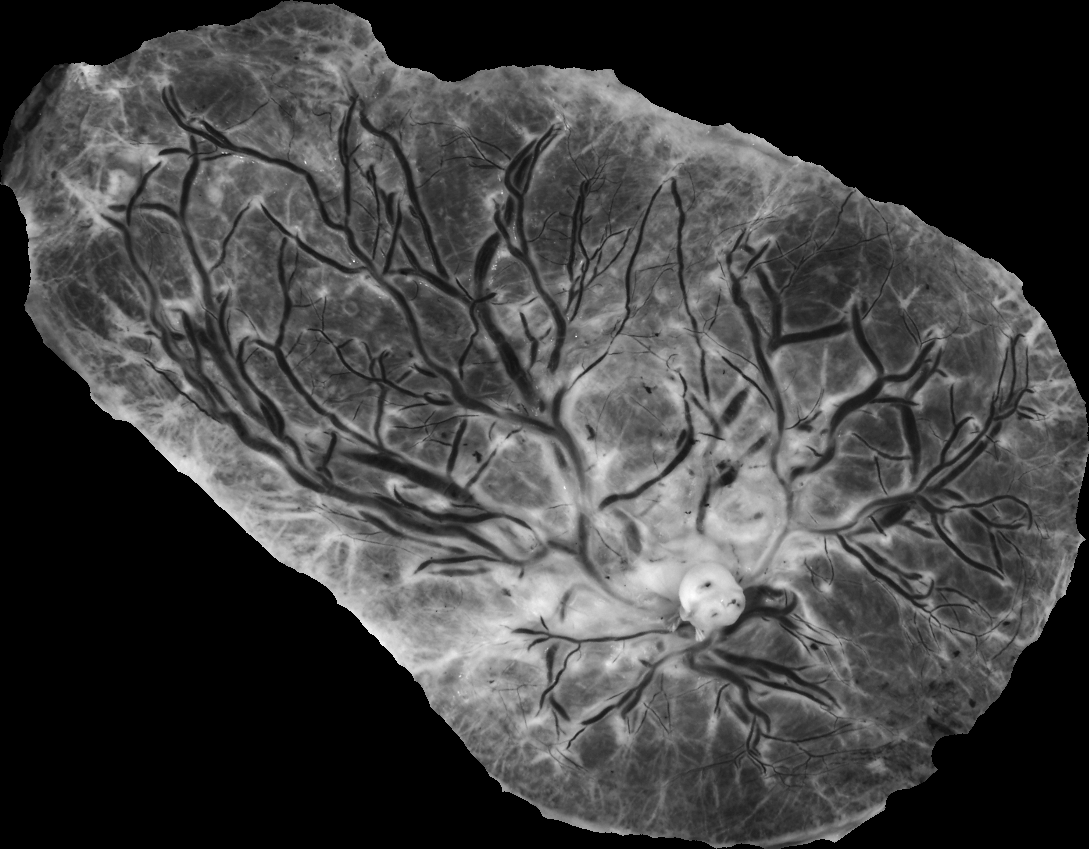
\includegraphics[width=0.48\linewidth]{qthresh_demo_img}} \;
		\subfloat{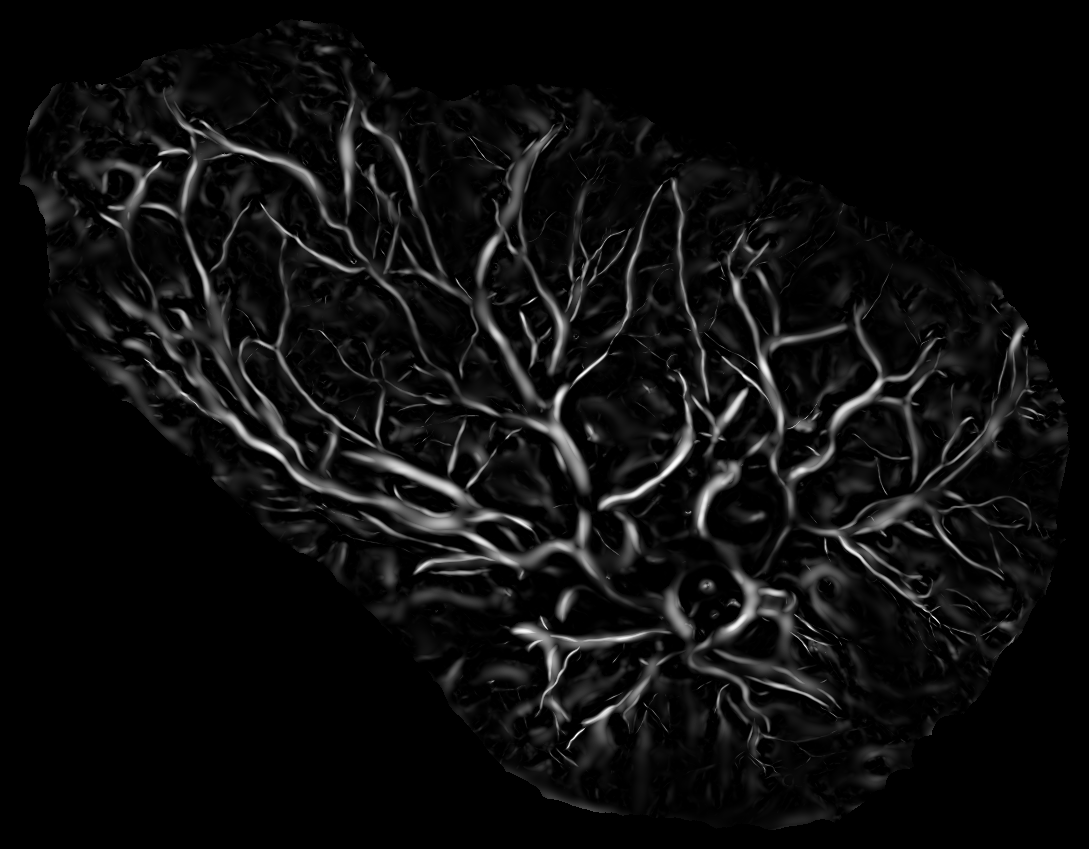
\includegraphics[width=0.48\linewidth]{qthresh_demo_Fmax}} \\
		\subfloat{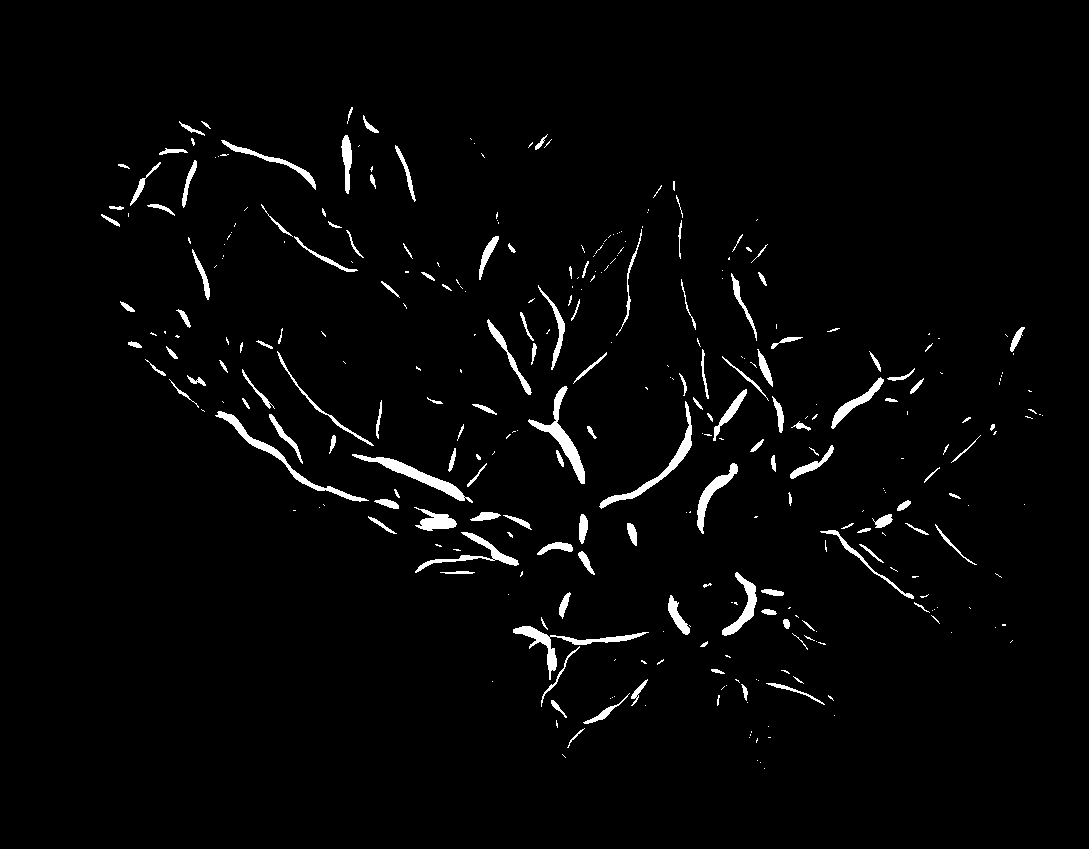
\includegraphics[width=0.48\linewidth]{qthresh_demo_q95}} \;
		\subfloat{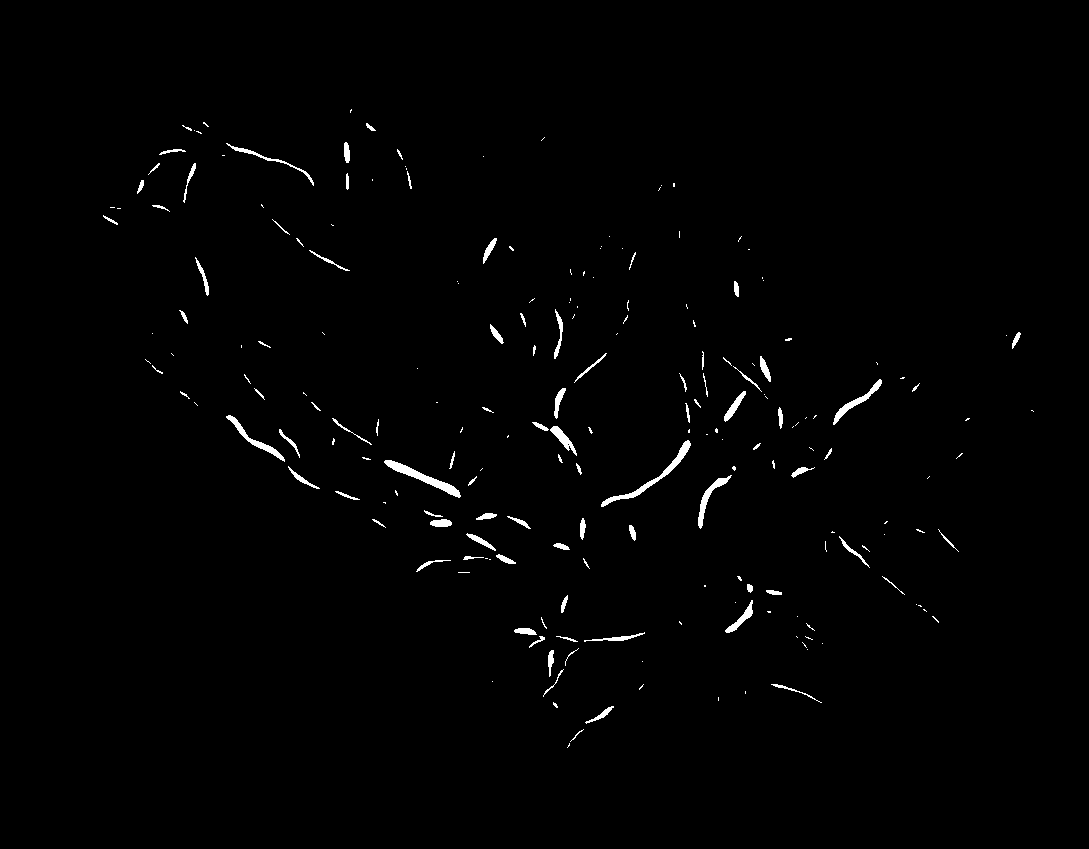
\includegraphics[width=0.48\linewidth]{qthresh_demo_q98}} \\
		\caption{Nonzero-percentile thresholding of \Vmax}.
		\label{fig:qthresh_demo}
	\end{figure}

	We will discuss alternatives methods of aggregating results from our multiscale method, as well as optimal values for parameters and scales
	in \cref{ch:implementations}. As a final note, we admit that any future extensions of this work (as will be discussed in \cref{ch:conclusion}) should not hold too much stock in this thresholded result, and analyzing the 
	raw vesselness score \cref{eq:Vmax}, or even
	the un-merged scale-wise scores, would be far more
	rewarding.    
	

All that remains to describe mathematically is how to actually calculate the derivatives of our images and deal with the ultimately discrete nature of our samples.    